\chapter{Design} \label{design}
In the following Section, the design decisions for this thesis are presented. The literature research revealed different interesting and promising approaches, but the most convincing and matured approach in the survey findings was the one by \cite{Banadaki_DetectingMalicousDoHTrafficinDNSUsingML} and \cite{BehnkeEtAl_FeatureEngineeringMLModelMaliciusDoHTraffic}. The layer approach, where in the first layer the DoH traffic is detected and in the second layer the malicious traffic is detected is a very convincing and inspiring work. Additionally the feature analysis and the proposal of the best performing ML model of \cite{BehnkeEtAl_FeatureEngineeringMLModelMaliciusDoHTraffic} is highly accurate. In terms of the feature selection, \cite{BehnkeEtAl_FeatureEngineeringMLModelMaliciusDoHTraffic}'s work suited very well to the work of all the references found in the previous chapter. Therefore this work is strongly based to their work.

For the detection of malicious DoH traffic the two layered approach that \cite{Banadaki_DetectingMalicousDoHTrafficinDNSUsingML} found will be approached, where the first layer separates DoH traffic from classic DNS traffic and the second layer detects malicious traffic and separate it from benign traffic. According to the findings of \cite{BehnkeEtAl_FeatureEngineeringMLModelMaliciusDoHTraffic}, the machine learning model that will do the detection will be the Light Gradient Boosting Machine, and for each layer, the 21 most important features according to the results of the statistical tests will be involved. Finally, the data for the default data-sets will be taken from \cite{montazerishatoori2020anomaly}, whereas it will be built according to the work of \cite{Banadaki_DetectingMalicousDoHTrafficinDNSUsingML} with two data-sets for each layer and with 40'000 data points for each data-set. 

The mentioned works will not be adopted exactly, since all those works were written in Python. SecGrid is mainly written in Javascript, therefore the feature extraction will be implemented also in Javascript to assure the compatibility. For the .pcap file analysis, node-pcap implemented in Javascript will be used instead of Scapy (Python), which possibly needs to be adjusted to be able to extract all the desired features.

The outline of this Chapter is as follows: first the data-set \cite{CIRA-CIC-DoHBrw-2020}, which provides the training data for this thesis is presented. The next two Sections describe how the traffic is filtered for HTTPS and how the TCP-flows are formed into clumps. The Section Feature Extraction presents all the features that are extracted from the TCP-clumps including their computations. In the next Section it is shown how the training data-sets are composed. The Section Light Gradient Boosting Machine presents the ML model that is used in this thesis and finally, the Section Architecture shows how all the presented parts are composed such they result in a working prototype. 

\section{Data-Set} \label{dataset}
For this thesis, the data-set created by \cite{montazerishatoori2020anomaly} and found at \cite{CIRA-CIC-DoHBrw-2020} is used. The data-set was created by using HTTPS traffic flows with two levels of distinct labels. The first level is assembled by normal HTTPS traffic and tunneled DoH traffic, the second level consists of benign DoH traffic and malicious DoH traffic. Figure \ref{fig:data_set} shows the illustration of how the data was collected. The traffic was collected by capturing HTTPS traffic from the web browsers \textit{Google Chrome} and \textit{Mozilla Firefox}. Using the browsers, he visited a set of the top 10'000 web sites of \textit{Alexa} to collect non-DoH-traffic data. Benign DoH-traffic data was collected by configuring both browsers to only use DoH connections instead of DNS traffic. To collect malicious DoHtraffic data, \cite{montazerishatoori2020anomaly} deployed a network that simulates malicious DoH tunneling scenarios.

After analyzing some of the PCAP-files contained in this data-set in Wireshark a surprising observation was made. Wireshark provides the function to filter one single TCP-flow. With this function it became visible that many TCP-flows are not ended correctly with the double FIN-ACK packet sequence like it was shown in chatpter \ref{tcp} and were just interrupted. Also checking the successor PCAP-file did not show any end of TCP-flows of the predecessor file. But as \cite{Blog_ClosingTCPSession} stated, it can be totally normal in the real world that TCP connections can be interrupted abruptly. This finding makes the approach of malicious DoH traffic detection of this thesis even more reliable and accurate and appropriate for a real world problem. As a consequence, each TCP-flow in the data-set that is not ending will be ended manually at the end of each PCAP file and a flag will be handed over to the feature collection. Since this problem is not handled in any of the references, it can be a limitation of all these works that is tried to be solved in this thesis.

\begin{figure} [h]
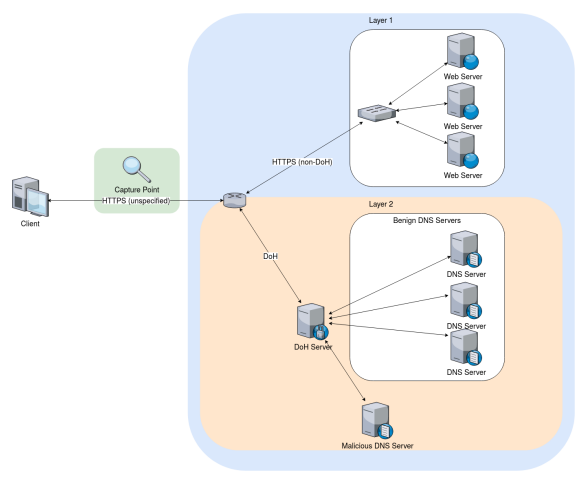
\includegraphics[scale=0.85]{images/data_set.PNG}
\centering
\caption{Illustration of the Collection of the Data by \cite{montazerishatoori2020anomaly}}
\label{fig:data_set}
\end{figure}

\section{Clumping} \label{clumping}
Before starting a complete analysis, some data can already be filtered. As mentioned in Section \ref{doh}, DoH works only on the HTTPS protocol, which only operates on port 443. Therefore only flows whose source port or destination port are port 433 will be considered further, every other flow which has nothing to do with the HTTPS port will be dropped.

\cite{montazerishatoori2020anomaly} had the idea of a clumping process in which he merged packets of a same flow. To ensure that only packets of one flow are in this clump, he uses a timeout which limits the time interval of the packets, i.e. each packet whose timestamp exceeds the timeout is automatically put into the next clump. In this thesis another clumping approach is followed (Figure \ref{fig:clumping}). A DoH connection has always on single TCP flow, therefore one clump will be built with one entire TCP flow. The advantage of such a clumping process is that not every single packet data sequence has to be forwarded, but only a summary of the whole TCP flow, which saves a lot of memory capacity. Another advantage of this clumping process is that it allows to extract statistical features, e.g. the median of the packet times in the clump etc. This process will be declared in the next Section.

In the Section \ref{dataset}, the problem of the non-ending flows was discussed. It was also pointed out that those flows are considered, too. The pragmatic solution for this is that if the PCAP file is over and the flow is still open, the flow is closed manually and the flag \textit{Status} will be passed as \textit{Open}. For the flows which are closed correctly the flag \textit{Status} will be passed as \textit{Closed}.

\begin{figure} [h]
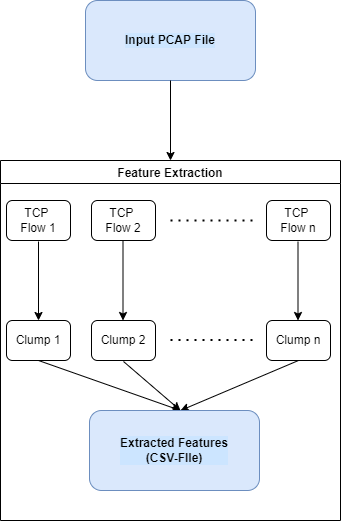
\includegraphics[scale=0.45]{images/clumping.png}
\centering
\caption{Illustration of the Clumping Process}
\label{fig:clumping}
\end{figure}

\section{Feature Extraction} \label{feature_extraction_design}
The feature extraction is done using the data-set \cite{CIRA-CIC-DoHBrw-2020}, whereas the extracted features rely strongly to the features \cite{montazerishatoori2020anomaly} computed and as already mentioned in Section \ref{clumping}, one clump consists of one TCP flow, from which all the features are extracted and computed. Statistical features are all computed with the same eight metrics, presented in Section \ref{stat_met}. Header features of every flow are extracted according to the features presented in Section \ref{head_feat}. The core features, which need to be computed, are presented in Sections \ref{pack_length}, \ref{pack_time}, and \ref{pack_resp}. Finally, the new found features in this thesis are presented in Section \ref{new_feat}. Totally, 40 features are presented in this Section.

\subsection{Statistical Metrics} \label{stat_met}
The statistical metrics used for the features in this work repeat for every property of a TCP-flow (\textit{packet length}, \textit{packet time}, and \textit{packet request/ response time}), therefore they are presented in this separate Section. All the metrics are derived from \cite{ross2010statistics} and summarized in Table \ref{tab:stat_met}. The following metrics all consider the data-set $x_{1}+x_{2}+\cdots+x_{n}$, where $x_{1}$ is the first entry of the data-set and $x_{n}$ is the last entry of the data-set. $n$ is considered the highest index in the data-set. If the equation requires modifications on the data-set, they are mentioned separately in the respective Section. 

\subsubsection{Mean}
The mean \cite{ross2010statistics} $\bar{x}$ (equation \ref{eq:mean}) or also the \textit{sample mean} indicates the center of a data-set, or in other words the arithmetic average of a sample. 

\begin{equation}
\bar{x} = \frac{\sum\nolimits_{i=1}^N}{x_{i}} = \frac{x_{1}+x_{2}+\cdots+x_{n}}{n}
\label{eq:mean}
\end{equation}

\subsubsection{Median}
The median \cite{ross2010statistics} $m$ (equations \ref{eq:median_odd} and \ref{eq:median_even}) indicates the middle of data-set, but unlike the mean it is not affected by extreme values. It is defined as follows:

Consider the ordered data-set $x_{1}+x_{2}+\cdots+x_{n}$ starting from the smallest $x_{1}$ value and ending at the biggest value $x_{n}$.

If \textit{n} is odd, then the median is the middle value of the ordered data-set.

\begin{equation}
m=x_{\frac{n}{2}+0.5}
\label{eq:median_odd}
\end{equation}

If \textit{n} is even, then the median is the average of the two middle values of the ordered data-set:
\begin{equation}
m=\frac{x_{\frac{n}{2}}+x_{\frac{n}{2}+1}}{2}
\label{eq:median_even}
\end{equation}

\subsubsection{Mode}
The $mode$ \cite{ross2010statistics} is indicates the value that occurs the most in the data-set and is therefore another indicator for the central tendencies of the data-set. If there is no unique value that occurs the most, then sequence of all values that occur the most indicated the \textit{modal values}.

\subsubsection{Variance}
The variance $s^2$ \cite{ross2010statistics} (equation \ref{eq:variance}) is the "average" of the summed squared differences between each value of the data-set and the mean of the data-set. It is no quiet the average, since the sum is no divided by $n$ but rather by $n-1$. The variance considers the spread tendencies of the data-set.

\begin{equation}
s^{2}=\frac{\sum\limits_{i=1}^N (x_{i}-\bar{x})^2}{n-1}
\label{eq:variance}
\end{equation}

\subsubsection{Standard Deviation}
The standard deviation $s$ \cite{ross2010statistics} (equation \ref{eq:std_dev}) is an indicator for the spread of the data-set. It is the positive square root of the variance.

\begin{equation}
s=\sqrt{\frac{\sum\limits_{i=1}^N (x_{i}-\bar{x})^2}{n-1}}
\label{eq:std_dev}
\end{equation}

\subsubsection{Coefficient of Variation}
The coefficient $CV$ \cite{jain2021statisticsEconomics} (equation \ref{eq:coeff}) of variation is used to compare the two different metrics standard deviation and mean multiplied. It is computed by dividing the standard deviation by the mean and multiplying it by 100.

\begin{equation}
CV = s/\bar{x}*100
\label{eq:coeff}
\end{equation}

\subsubsection{Skew from Mode}
The Skew from Mode or also Pearson's first coefficient of skewness $S_{kp1}$ \cite{awasthi2013statistics} (equation \ref{eq:skew_mode}) is used to compare the symmetry of two or more distributions of data-sets. It is computed by subtracting the $mode$ from the mean $m$ and dividing the difference by the standard deviation $s$.

\begin{equation}
S_{kp1} = \frac{\bar{x}-mode}{s}
\label{eq:skew_mode}
\end{equation}

\subsubsection{Skew from Median}
The Skew from Median or also Pearson's second coefficient of skewness $S_{kp2}$ \cite{awasthi2013statistics} (equation \ref{eq:skew_median}) is used to compare the symmetry of two or more distributions of data-sets. It is computed by three times the difference between the mean and the median divided by the standard deviation.

\begin{equation}
S_{kp2} = \frac{3*(\bar{x}-m)}{s}
\label{eq:skew_median}
\end{equation}

\begin{center}
\begin{tabular}{ |l|l|l| }
\hline
No. & Metric & Format of Feature \\
\hline
1 & Mean & \textit{float} \\
\hline
2 & Median & \textit{float} \\
\hline
3 & Mode & \textit{int} \\
\hline
4 & Variance & \textit{float} \\
\hline
5 & Standard Deviation & \textit{float} \\
\hline
6 & Coefficient of Variation & \textit{float} \\
\hline
7 & Skew from Mode & \textit{float} \\
\hline
8 & Skew from Median & \textit{float} \\
\hline
\end{tabular}
\captionof{table}{Statistical Metrics}
\label{tab:stat_met}
\end{center}

\subsection{Header Features} \label{head_feat}
The identifying header features are the features \textit{Source IP}, which is the IP of the client, \textit{Destination IP}, which is the IP of the server, \textit{Source Port}, which is the port of the client, and \textit{Destination Port}, which is the port of the server. All the four features have the format \textit{string}. Since these features are only passed to the set of extracted features for informational purposes and are not further used, the format \textit{string} is appropriate. The feature \textit{Duration} indicates the total period the connection lasted and has the format \textit{float}. The two features \textit{Flow Bytes Sent} and \textit{Flow Bytes Received} sum up the total number of Bytes sent from the client to the server, or received from the client and sent by the server respectively. Both the features have format \textit{int}. The \textit{Flow Sent Rate} (equation \ref{eq:flow_sent_rate}) is computed by dividing the total number of sent Bytes by the client by the duration it lasted until the next packet was sent. Accordingly, the \textit{Flow Received Rate} (equation \ref{eq:flow_recv_rate}) is computed by dividing the total number of received Bytes by the client by the duration it lasted until the next packet was received. Both the features have the format \textit{float}. Figure \ref{tab:head_feat} sums up all the features presented in this Section.

\begin{equation}
\textit{\textit{Flow Sent Rate}} = \frac{Total \; Number \; of \; sent \; Bytes}{Time \; last \; sent \; Packet - Time \; first \; sent \; Packet}
\label{eq:flow_sent_rate}
\end{equation}

\begin{equation}
\textit{\textit{Flow Received Rate}} = \frac{Total \; Number \; of \; received \; Bytes}{Time \; last \; received \; Packet - Time \; first \; received \; Packet}
\label{eq:flow_recv_rate}
\end{equation}

\begin{center}
\begin{tabular}{ |l|l|l| }
\hline
No. & Feature & Format \\
\hline
1 & Source IP & \textit{string} \\
\hline
2 & Destination IP & \textit{string} \\
\hline
3 & Source Port & \textit{string} \\
\hline
4 & Destination Port & \textit{string} \\
\hline
5 & Duration & \textit{float} \\
\hline
6 & Flow Bytes Sent & \textit{int} \\
\hline
7 & Flow Bytes Received & \textit{int} \\
\hline
8 & Flow Sent Rate & \textit{float} \\
\hline
9 & Flow Received Rate & \textit{float} \\
\hline
\end{tabular}
\captionof{table}{Header Features}
\label{tab:head_feat}
\end{center}

\subsection{Packet Length Features} \label{pack_length}
Packet length features are computed from the set of all extracted sizes (in Bytes) of every packet in one clump and by using the metrics presented in Section \ref{stat_met}. Table \ref{tab:length_feat} summarizes all eight packet length features. 

\begin{center}
\begin{tabular}{ |l|l| }
\hline
No. & Feature \\
\hline
1 & Packet Length Mean \\
\hline
2 & Packet Length Median \\
\hline
3 & Packet Length Mode \\
\hline
4 & Packet Length Variance \\
\hline
5 & Packet Length Standard Deviation \\
\hline
6 & Packet Length Coefficient of Variance \\
\hline
7 & Packet Length Skew from Median \\
\hline
8 & Packet Length Skew from Mode  \\
\hline
\end{tabular}
\captionof{table}{Packet Length Features}
\label{tab:length_feat}
\end{center}

\subsection{Packet Time Features} \label{pack_time}
Packet time features are computed from the set of all extracted durations (in seconds) between the first packet was sent until the actual packet is sent in one clump and by using the metrics presented in Section \ref{stat_met}. Table \ref{tab:time_feat} summarizes all eight packet time features. 

\begin{center}
\begin{tabular}{ |l|l| }
\hline
No. & Feature \\
\hline
1 & Packet Time Mean \\
\hline
2 & Packet Time Median \\
\hline
3 & Packet Time Mode \\
\hline
4 & Packet Time Variance \\
\hline
5 & Packet Time Standard Deviation \\
\hline
6 & Packet Time Coefficient of Variance \\
\hline
7 & Packet Time Skew from Median \\
\hline
8 & Packet Time Skew from Mode  \\
\hline
\end{tabular}
\captionof{table}{Packet Time Features}
\label{tab:time_feat}
\end{center}

\subsection{Packet Request/ Response Time Features} \label{pack_resp}
For packet request/ response features, first the difference of sending a packet from the client until the answer of the server was received (in seconds) is computed. From this difference, the metrics presented in Section \ref{stat_met} are computed. Table \ref{tab:resp_feat} summarizes all eight packet request/ response features. 

\begin{center}
\begin{tabular}{ |l|l| }
\hline
No. & Feature \\
\hline
1 & Packet Request/ Response Time Mean \\
\hline
2 & Packet Request/ Response Time Median \\
\hline
3 & Packet Request/ Response Time Mode \\
\hline
4 & Packet Request/ Response Time Variance \\
\hline
5 & Packet Request/ Response Time Standard Deviation \\
\hline
6 & Packet Request/ Response Time Coefficient of Variance \\
\hline
7 & Packet Request/ Response Time Skew from Median \\
\hline
8 & Packet Request/ Response Time Skew from Mode  \\
\hline
\end{tabular}
\captionof{table}{Packet Request/ Response Time Features}
\label{tab:resp_feat}
\end{center}

\subsection{Novel Features} \label{new_feat}
In this thesis, new additional features to the features \cite{montazerishatoori2020anomaly} developed are introduced. The \textit{State} is a flag that indicates if a TCP session was closed or not. As seen in chapter \ref{tcp}, the initiator of the closure of a TCP session could either be the client or the server. If it is \textit{closed} it means that the TCP session was closed and so the flag receives the value 1. If it is \textit{open} it means that the TCP session was not closed correctly and so the flag receives the value 0. The values 0 and 1 in format \textit{int} are chosen to be numerically since the ML model is not able to process string-values. The feature \textit{Number of Application Packets Sent} indicates the total number of packets sent by the client in the TCP flow, the feature \textit{Number of Application Packers Received} correspondingly indicates the number of packets recieved by the client in the TCP flow. Both the features have the format \textit{int}. 

The feature \textit{Number of ACKs Sent} sums up the total number of ACK packets sent by the client in the TCP flow, the feature \textit{Number of ACKs Received} accordingly is the summed up total number of ACK packets received by the client in this flow. Both the features have the format \textit{int}. The feature \textit{Number of Retransmits Sent} sums up the total number of retransmission packets sent by the client in the TCP flow, the feature \textit{Number of Retransmits Received} sums up the total number of retransmission packet received by the client in the TCP flow. Finally, the the feature \textit{Total Packet length} indicates the summed up length of all packets sent and received by the client in one flow. Table \ref{tab:new_feat} sums up all the features introduced in this Section.

\begin{center}
\begin{tabular}{ |l|l|l| }
\hline
No. & Feature & Format \\
\hline
1 & State & \textit{int} \\
\hline
2 & Number of Application Packets Sent & \textit{int} \\
\hline
3 & Number of Application Packets Received & \textit{int} \\
\hline
4 & Number of ACKs Sent & \textit{int} \\
\hline
5 & Number of ACKs Received & \textit{int} \\
\hline
6 & Number of Retransmits Sent & \textit{int} \\
\hline
7 & Number of Retransmits Received & \textit{int} \\
\hline
8 & Total Packet Length & \textit{int} \\
\hline
\end{tabular}
\captionof{table}{New Features compared to the Work of \cite{montazerishatoori2020anomaly}}
\label{tab:new_feat}
\end{center}

\section{Training Data-Sets} \label{training_ds}
Since the ML model is trained two times (Layer 1 and Layer 2), it is also necessary to have two different training data-sets. Layer 1 conducts the classification into non-DoH and DoH traffic, therefore the data contained in the training set for Layer 1 (TSL1) contains an equal amount of DoH traffic and non-DoH traffic, whereas the DoH traffic is split equal into benign an malicious traffic. \cite{Banadaki_DetectingMalicousDoHTrafficinDNSUsingML} composed his training data-sets with 40'000 data points, thus the total amount of data contained TSL1 is also 40'000 data points. The traffic data is marked with a flag called \textit{doh} for indicating the ML model if the data is DoH traffic or non-DoH traffic. If the flag has the value 0, this means that the traffic is non-DoH traffic. If the flag has the value 1, this means that the traffic is DoH traffic. TSL1 has its feature ordered according to \cite{BehnkeEtAl_FeatureEngineeringMLModelMaliciusDoHTraffic} in Figure \ref{fig:feature_importance} on the left side, without the red marked features, but with additionally the new features introduced in this thesis appended at the end.

Layer 2 conducts the classification into benign traffic and malicious traffic, therefore the training set for Layer 2 (TSL2) contains equally split traffic into benign and malicious traffic. The the malicious traffic is equally split into three different parts: malicious traffic from the tunnel tools \textit{iodine}, \textit{DNS2TCP}, and \textit{DNScat2}. The total amount of data points in TSL2 is again 40'000 data points. The traffic is marked with a flag called \textit{malicious}. If the flag has the value 0, this means that the traffic is benign. If the flag has the value 1, this means that the traffic is malicious. TSL2 has its feature ordered according to \cite{BehnkeEtAl_FeatureEngineeringMLModelMaliciusDoHTraffic} in Figure \ref{fig:feature_importance} on the right side, without the red marked features, but with additionally the new features introduced in this thesis appended at the end.

\section{Light Gradient Boosting Machine} \label{LGBM}
Light Gradient Boosting Machine (LGBM) \cite{ke2017lightgbm} is a sub-type of Gradient Boosting Decision Tree (GBDT). It is fast, efficient and has an excellent scalability when the number of features is high and the amount of data is large. To solve this problem, it uses \textit{Gradient-based One-Side-Sampling} (GOSS) and \textit{Exclusive Feature Bundling} (EFB). GOSS introduces a native gradient weight handling, which means that instances were not trained as successful as other instances contribute more to the information gain than the well-trained instances during the training process. EFB clusters mutually exclusive features into one single feature to reduce the amount of features. Mutually exclusive features are two or more features that never take non-zero values when at the same time another feature takes a non-zero value. In this thesis, LGBM is used for both layers of the malicious DoH traffic detection process due to its promising characteristics. 

\section{Architecture} \label{architecture}
After all design decisions are completed, it is now time to show how all the previously introduced parts work together in the SecGrid prototype for malicious DoH traffic detection. Figure \ref{fig:changed_arch} shows the architecture of SecGrid. The tow part which have to be adjusted are the Protocol Parser and the Feature Extractors, which are marked green in the Figure. The whole pipeline will be implemented there, all the other parts will not be affected. The Protocol Parser needs to be adjusted since currently it only parses entire PCAP-files, but the approach of this thesis demands it to parse TCP-flows. Therefore a whole new TCP-flow handling will be implemented.

\begin{figure} [h]
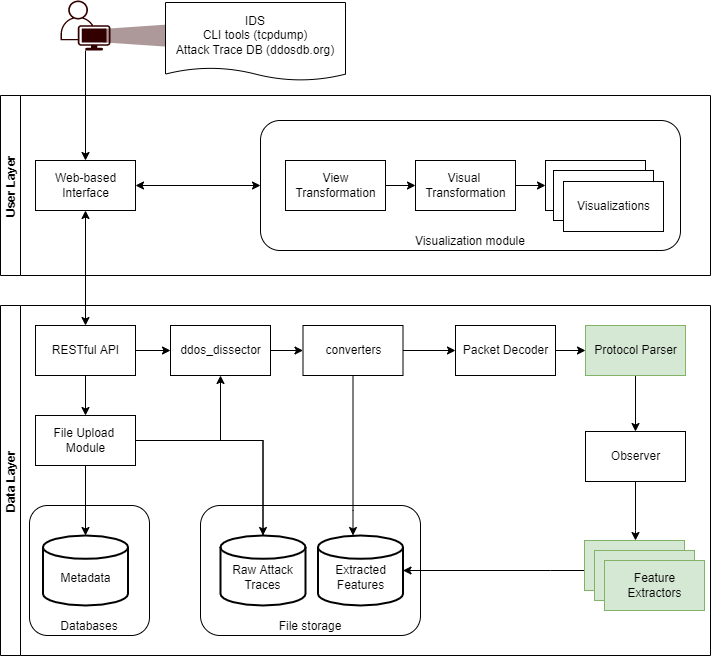
\includegraphics[scale=0.6]{images/changed_architecture.png}
\centering
\caption{Components to be adapted}
\label{fig:changed_arch}
\end{figure}

The Feature Extractors will be adjusted according to Figure \ref{fig:2_layers}, which shows the whole pipeline of the new process. The PCAP-file to be analyzed is given as a input to SecGrid, which first will parse the file into the individual TCP-flows. The Feature Extraction extracts all the demanded features (see Section \ref{feature_extraction_design}) and weited them into the respective clump. The clumps in turn will then be written into a CSV-file. As soon as every flow/ clump is extracted from the input file, the finished CSV-file with all the feature information is then handed over to the Classification. The Classification is split into two parts (layers): the first part Separates DoH traffic from non-DoH traffic and hands over only the DoH traffic clumps to the second part. In the second part, the DoH traffic is analyzed and malicious DoH traffic is identified. The output of SecGrid is then a file with classified DoH traffic, whereas the user will be noticed if there is malicious traffic recorded in the input PCAP-file.

\begin{figure} [h]
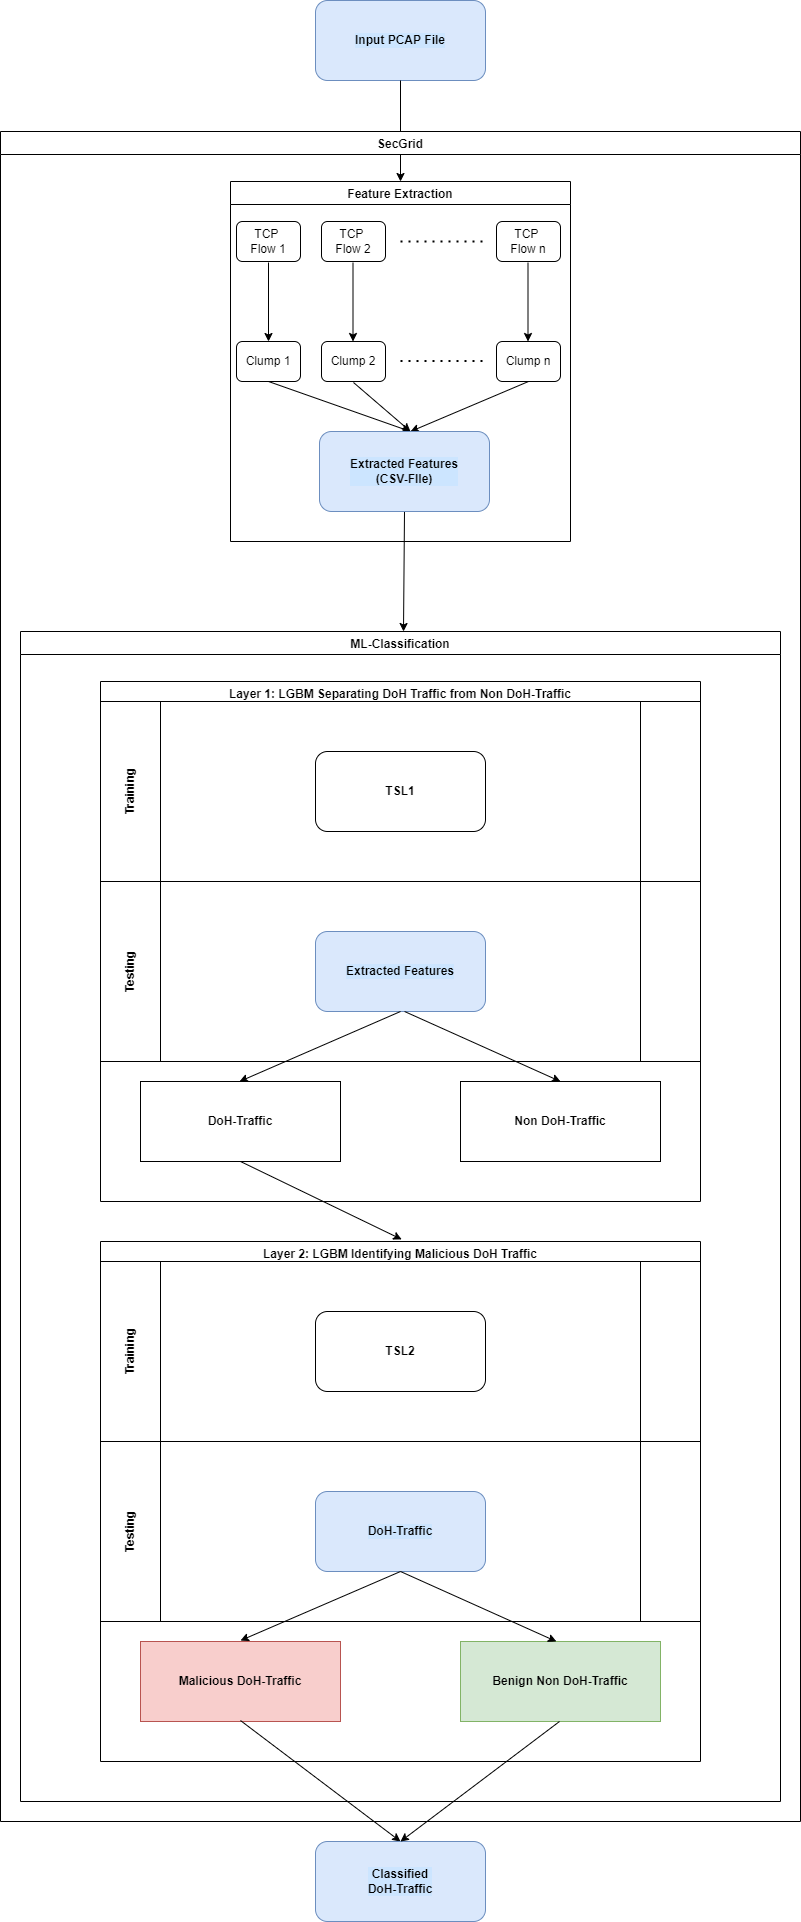
\includegraphics[scale=0.34]{images/2_layers.png}
\centering
\caption{Illustration of the whole Classification Process of an Input PCAP File}
\label{fig:2_layers}
\end{figure}
